\saltoPag%
\section{UNIDAD 2}
    \subsection{Experimentos y teorías}
        \begin{center} \textcolor{red}{\underline{Exp. De Millikan}} \end{center}
        \indent Determinación de la masa específica del electrón.
        \begin{center} 
            \begin{tabular}{|| c | c ||}
                \hline
                \textbf{Concepto}    &   \textbf{Valores}     \\
                \hline
                \hline
                Relación carga/masa  &   $-1,76 \times 10^8 C/g$ \\
                \hline
                Carga del $e^-$      &  $-1.60 \times 10^{-19} C$ \\
                \hline
                Masa del $e^-$       &  $9,10 \times 10^{-28} g$ \\
                \hline
            \end{tabular}
        \end{center}

        \begin{center} 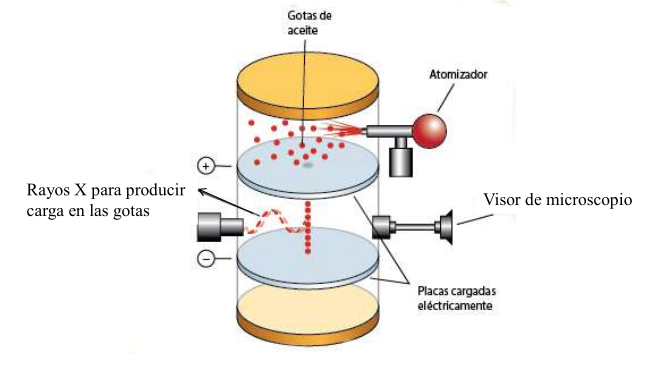
\includegraphics[width=8cm]{./imagenes/experienciaMIllikan.png} \end{center}

        \begin{center} \textcolor{red}{\underline{Radiactividad}} \end{center}
            \begin{center} 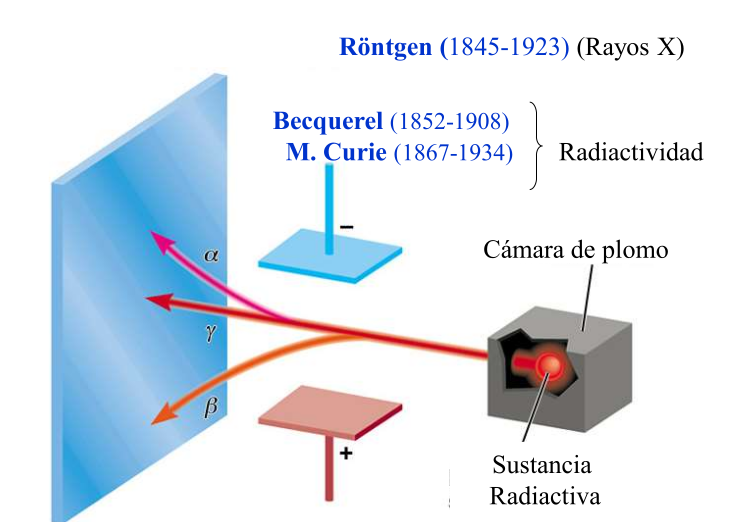
\includegraphics[width=8cm]{./imagenes/radiactividadExperimento.png} \end{center}

        \begin{center} \textcolor{red}{\underline{Modelo de Thomson}} \end{center}
            \begin{center} 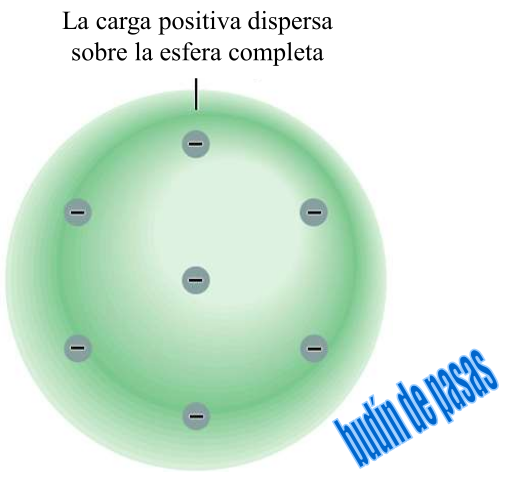
\includegraphics[width=7cm]{./imagenes/modeloDeThomson.png} \end{center}
        
        \begin{center} \textcolor{red}{\underline{Exp. De Rutherford}} \end{center}
            \begin{enumerate} 
                \item La carga positiva de un átomo está concentrada en su núcleo.
                \item El protón ($p$) tiene una carga $+$, el electrón tiene carga $-$.
                \item La masa del protón es 1840 $\times$ masa del $e^-$ ($1.67 \ times 10^{-24}g$).
            \end{enumerate}

            \begin{center} 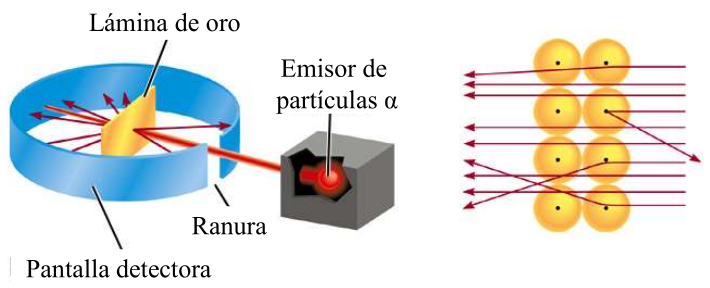
\includegraphics[width=8cm]{./imagenes/experimentoRutherford.png} \end{center}

        \begin{center} \textcolor{red}{\underline{El neutrón}} \end{center}
            \begin{center} 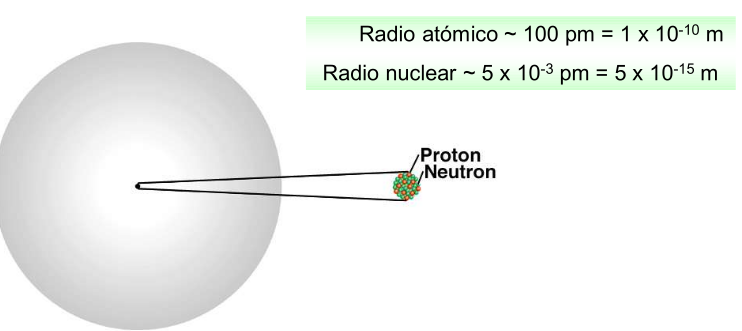
\includegraphics[width=7cm] {./imagenes/neutron.png} \end{center}

        \begin{center} \textcolor{red}{\underline{Exp. De Chadwick}} \end{center}
            \indent Se bombardeo una delgada lámina de $Be$ con partículas $\alpha$, el metal emitió una radiación de muy alta energía, similar a los rayos $\gamma$. Posteriormente se demostró que eran neutrones.
            
            \begin{tabular}{|| c | c | c | c ||}
                \hline
                \textbf{\scalebox{0.8}{Partícula}}  &   \textbf{\scalebox{0.8}{Masa(g)}}   &   \textbf{\scalebox{0.8}{Carga(C)}}    &   \textbf{\scalebox{0.8}{Unidad de carga}} \\
                \hline
                Electrón            &   $9,109 \times 10^{-28}$     &   $-1,602 \times 10^{-19}$   &   $-1$    \\
                \hline
            \end{tabular}
            
        

